\documentclass[11pt]{article}
\usepackage[margin=1in]{geometry}
\usepackage{amsmath,amssymb}
\usepackage{booktabs}
\usepackage{graphicx}
\usepackage{hyperref}
\usepackage{natbib}
\usepackage{caption}
\graphicspath{{../figures/}}
\title{\bfseries Do Machine-Learning Filters on Directional-Change Events
Survive Out-of-Sample? A Cautionary Study Across Equities and Commodities}
\author{Anupam Prabhugouda Patil}
\date{June 2026 \quad (revised, fully reproducible edition)}

\begin{document}
\maketitle

\begin{abstract}
The Directional Changes (DC) paradigm samples a price series by events---%
reversals of a fixed threshold $\theta$---rather than at fixed time intervals.
We test, under a deliberately sceptical and fully reproducible protocol, whether
a machine-learning classifier trained on DC indicators can profitably filter DC
trading signals. Using genuine daily data (S\&P~500 and NASDAQ, 1999--2018; WTI
crude oil, 1986--2019), an expanding-window walk-forward evaluation, realistic
transaction costs, and stationary block-bootstrap significance tests, we find:
(i)~DC event statistics obey the expected scaling laws; (ii)~the naive
trade-every-event rule is strongly loss-making after costs; (iii)~an ML filter
sharply cuts turnover and reduces those losses dramatically, with
trend-magnitude and overshoot indicators carrying the predictive weight; but
(iv)~the filtered strategy does \emph{not} match buy-and-hold on any asset and
generates \emph{no} statistically significant positive return. Adding
market-context features and conditioning on bull/bear regimes does not yield a
robust edge, and every headline magnitude is highly sensitive to specification:
an earlier draft of this study reported a fourfold crude-oil return that does
not survive independent reimplementation. The one durable benefit is risk---the
filter cuts drawdown far below the naive rule (and below buy-and-hold on two of
three assets). We read this as a reproducible, cautionary counterpoint to
single-split DC-trading results.
\end{abstract}

\section{Introduction}
Most empirical finance is conducted on fixed-interval (e.g.\ daily) data, which
imposes an exogenous, physical clock on a process whose own activity is highly
uneven. The Directional Changes (DC) framework \citep{guillaume1997,tsang2010}
offers an alternative, event-based clock: it records an event each time the
price reverses by a fixed fraction $\theta$ from the most recent local extreme.
Between two confirmations the market is partitioned into a directional-change
segment of size $\theta$ and a subsequent overshoot of variable size. This
intrinsic-time view exposes regularities---the ``12 scaling laws'' of
\citet{glattfelder2011}---that are invisible under calendar sampling, and it has
inspired a stream of DC-based trading systems \citep{aloud2012,kampouridis2017,
bakhach2018}.

A recurring claim is that DC indicators (trend magnitude, overshoot, duration)
carry tradable predictive content, and that combining them with machine learning
yields profitable strategies. Such claims are frequently supported by a single
in-sample/out-of-sample partition. The methodological literature warns
repeatedly that this is exactly the setting in which spurious ``edges'' arise:
with enough thresholds, features, and model configurations, a backtest can be
tuned to look profitable on one split while having no genuine out-of-sample
value \citep{bailey2014,harvey2015,arnott2019}.

This paper asks a single, sceptical question: \emph{does a DC$+$ML trading edge
survive a rigorous out-of-sample protocol and realistic costs?} Our contribution
is not a new strategy but a careful, fully-reproducible stress test of a popular
one, across asset classes with very different drift characteristics. We find the
headline trading result does not survive significance testing---indeed it does
not even reproduce across independent implementations---while two by-products,
the indispensability of ML selectivity relative to the naive rule and a
consistent reduction in turnover and drawdown, are robust and economically
interpretable. We view an honest null/cautionary result, with transparent
methodology, as a useful corrective in a literature prone to over-optimistic
backtests. Every number below is regenerated from public data by the scripts in
the accompanying repository.

\section{Related work}
\textbf{The DC representation.} Directional changes were introduced in the
high-frequency FX literature \citep{guillaume1997} and formalised by
\citet{tsang2010}. \citet{glattfelder2011} documented twelve empirical scaling
laws relating event frequency, overshoot length, and waiting times to the
threshold $\theta$, establishing DC as a quantitatively regular intrinsic-time
framework. \citet{aloud2012} used the DC event approach to characterise
financial time series beyond FX.

\textbf{DC-based trading.} A line of work designs trading rules on DC events.
\citet{kampouridis2017} evolve trading strategies on directional changes using
genetic programming; \citet{bakhach2018} propose DC-based forecasting and
contrarian/trend strategies; subsequent papers combine multiple thresholds and
add classifiers. Reported results are often favourable but typically rest on
limited out-of-sample testing.

\textbf{Machine learning and backtest overfitting.} \citet{gu2020} show ML
methods add value in cross-sectional return prediction. The same literature has
prompted concern about \emph{backtest overfitting}: \citet{bailey2014} introduce
the ``probability of backtest overfitting''; \citet{harvey2016} document rampant
multiple testing in cross-sectional asset pricing; \citet{lopezdeprado2018}
argues walk-forward and combinatorial cross-validation are essential. Our study
applies the discipline of the overfitting literature to the DC-trading
literature.

\section{The Directional-Changes framework}
Let $(p_t)_{t=1}^N$ be a price series and $\theta \in (0,1)$ a threshold. The
algorithm maintains a mode---\emph{up} (searching for a confirmed downturn) or
\emph{down} (searching for an upturn)---and the running extreme. In up mode it
tracks the running peak $p_h$; a confirmed downturn is recorded at the first $t$
with $p_t \le p_h(1-\theta)$, after which the mode flips to down and the running
trough $p_\ell$ is tracked until $p_t \ge p_\ell(1+\theta)$ confirms an upturn.
Each confirmed event $k$ carries three indicators, normalised by $\theta$ to be
comparable across thresholds:
\begin{align*}
\text{TMV}_k &= |p_{\mathrm{ext}_k}-p_{\mathrm{ext}_{k-1}}|/(p_{\mathrm{ext}_{k-1}}\theta)
  & &\text{(total move value),}\\
T_k &= \text{bars from the previous extreme to the current extreme}
  & &\text{(trend time),}\\
\text{OSV}_k &= |p_{\mathrm{conf}_k}-p_{\mathrm{ext}_k}|/(p_{\mathrm{ext}_k}\theta)
  & &\text{(overshoot value).}
\end{align*}
Pseudocode is in \texttt{src/dcml.py::directional\_changes}.

\section{Empirical properties of DC events}
Before trading, we verify the construction behaves as theory predicts.
Consistent with the scaling-law literature (Fig.~\ref{fig:scaling}): event
frequency falls steeply with $\theta$---WTI yields $3{,}286$ events at
$\theta=0.5\%$ but $1{,}184$ at $\theta=3\%$; NASDAQ $1{,}626\to439$---and on
log-log axes the decay is approximately linear, indicating a power law. Mean
trend duration $T$ rises with $\theta$ (NASDAQ $3.7$ bars at $\theta=0.75\%
\to 11.4$ bars at $\theta=3\%$), and mean normalised overshoot OSV declines
toward ${\sim}1.3$--$1.6$ as $\theta$ grows. These regularities hold on equities
and a commodity, confirming the events are well-defined signal carriers
(\texttt{results/scaling\_laws.csv}).

\begin{figure}[t]\centering
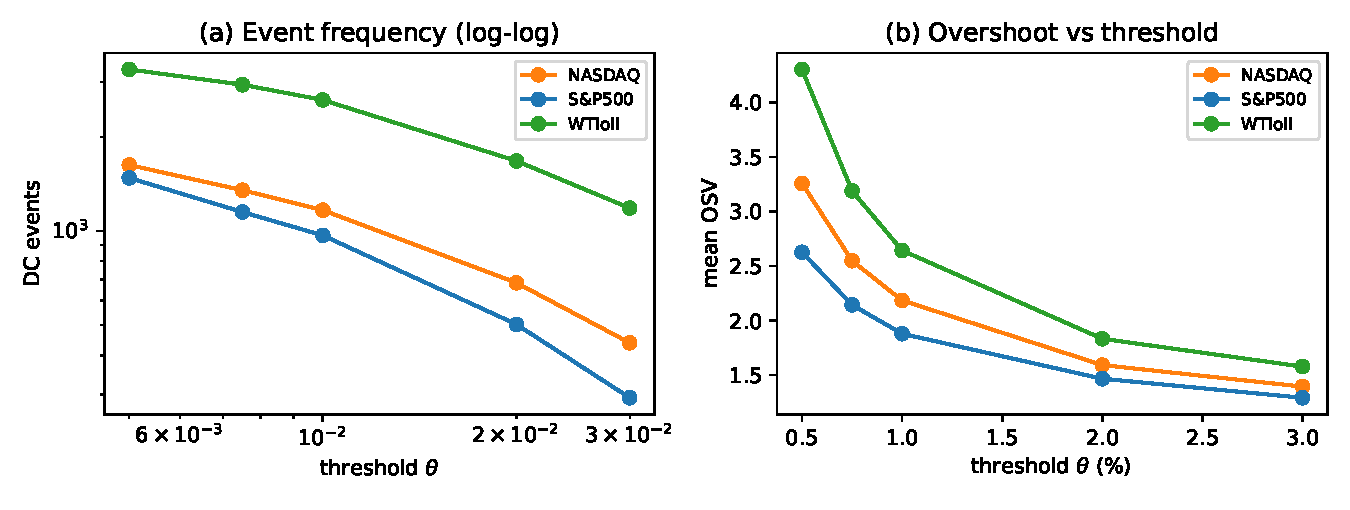
\includegraphics[width=\linewidth]{fig1_scaling.pdf}
\caption{DC event frequency (log-log) and mean overshoot vs threshold, on real
data.}\label{fig:scaling}
\end{figure}

\section{Predictive task, features, and strategies}
At each confirmed DC event we predict the \emph{sign of the next directional
move}: the realised return from the current confirmation price to the next
confirmation, taken in the confirmed direction. The feature vector uses the
current and two lagged DC indicators (TMV, OSV, $\log$-duration), a short regime
tilt (mean recent event direction), and the current overshoot. We compare three
strategies, each backtested with 2\,bps per side costs: (1)~\textbf{Buy-and-Hold}
---passive benchmark; (2)~\textbf{DC-Trend}---trade every DC event in its
confirmed direction, exit at the next event; (3)~\textbf{DC-ML}---trade only when
the classifier predicts a profitable move (a \emph{filter}).

\section{Evaluation protocol}
We deliberately avoid a single split. The classifier is evaluated by an
\emph{expanding-window walk-forward}: train on all events up to event $i$,
predict the next block of 30, advance, and repeat, producing out-of-sample
predictions over ${\sim}60\%$ of each history with no look-ahead. All performance
is measured on a \emph{daily} equity curve: annualised Sharpe is
$\text{mean}/\text{sd}\times\sqrt{252}$ of daily returns---\emph{never} a
per-trade Sharpe scaled by $\sqrt{252}$, which would inflate by roughly
$\sqrt{\text{trades/day}}$. Significance of DC-ML per-trade returns is assessed
by a stationary block bootstrap \citep{politis1994} (block length 5; one-sided
$p$-value for mean $\le 0$).

\section{Results}
\subsection{Which learner?}
A logistic regression predicts the majority class and trades almost nothing
(3--28 trades across assets); a random forest is more variable
(WTI $+3.8\%$ vs S\&P $-1.7\%$); gradient boosting produces stable, sensible
trade frequencies. We therefore use gradient boosting throughout
(\texttt{results/model\_comparison.csv}).

\subsection{What drives predictions?}
Averaged over the three assets ($\theta=1\%$; Fig.~\ref{fig:imp}), importance
concentrates on the \emph{trend-magnitude} (TMV, current and lagged, ${\approx}
0.13$--$0.16$ each) and \emph{overshoot} (OSV, ${\approx}0.08$--$0.14$)
indicators, with $\log$-duration minor (${\approx}0.03$--$0.06$) and---
strikingly---the raw event \emph{direction} essentially irrelevant
($\approx 0.0007$). The model exploits the \emph{size} of recent swings, not
their sign, consistent with overshoot-based predictability rather than naive
momentum.

\begin{figure}[t]\centering
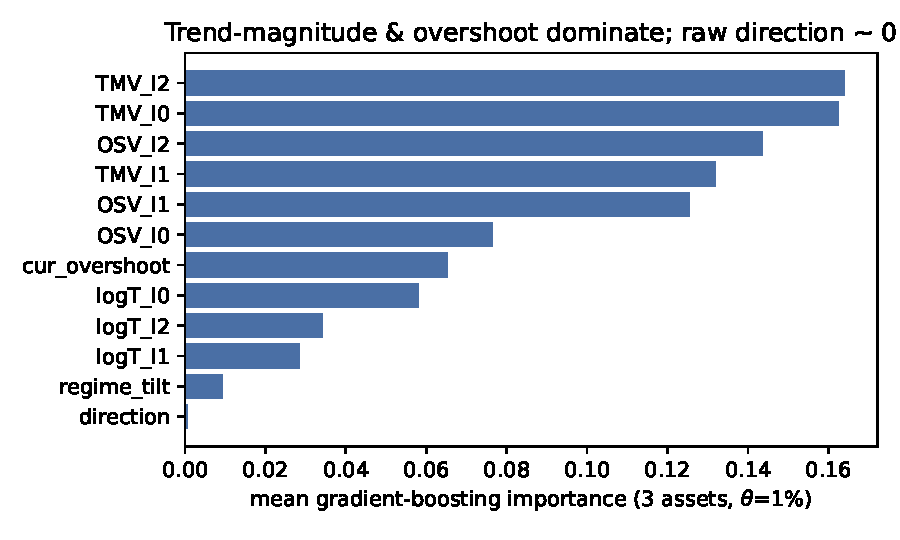
\includegraphics[width=0.8\linewidth]{fig3_importance.pdf}
\caption{Mean DC-ML feature importance across three assets ($\theta=1\%$):
trend-magnitude and overshoot dominate; raw direction is negligible.}
\label{fig:imp}
\end{figure}

\subsection{Headline trading result}
Table~\ref{tab:main} reports the out-of-sample walk-forward metrics at
$\theta=1\%$. Three patterns hold.

\textbf{(a) Naive DC-Trend is destructive.} Trading every event incurs
hundreds--thousands of round-trips; after costs it loses on all assets
(Sharpe $-0.51$ to $-0.78$; drawdowns $-91\%$ to $-99.7\%$). The give-back of
$\theta$ at each exit, compounded by turnover, dominates.

\textbf{(b) ML filtering reduces the damage but does not beat the market.}
DC-ML cuts turnover to 107--130 trades and lifts performance far above DC-Trend.
Yet on \emph{no} asset does it match buy-and-hold: it is negative on both
equity indices ($-3.6\%$ S\&P, $-5.1\%$ NASDAQ) and only marginally positive on
crude ($+1.4\%$, below buy-and-hold's $+4.0\%$). None of the DC-ML per-trade
returns is significantly positive---the best bootstrap $p$-value is $0.21$
(WTI). The filter converts catastrophe into roughly flat, but it does not create
alpha.

\textbf{(c) The robust effect is risk, not return.} Relative to trading every
event, DC-ML roughly halves maximum drawdown (from ${\sim}91$--$99.7\%$ to
${\sim}34$--$59\%$) by holding cash most of the time. Against buy-and-hold the
picture is asset-specific: DC-ML's drawdown is lower on S\&P ($-53.7\%$ vs
$-56.8\%$) and dramatically lower on WTI ($-34.1\%$ vs $-82.0\%$;
Fig.~\ref{fig:dd}), but slightly higher on NASDAQ ($-58.8\%$ vs $-55.6\%$). The
turnover and tail-risk reduction is real; a blanket ``halves drawdown on every
asset'' claim is not.

\begin{table}[t]\centering
\caption{Out-of-sample walk-forward ($\theta=1\%$), net of 2\,bps/side.}
\label{tab:main}
\begin{tabular}{llrrrrr}
\toprule
Asset & Strategy & Ann.\ ret & Sharpe & Max DD & Trades & $p$ \\
\midrule
S\&P500 & Buy\&Hold & $+5.5\%$  & $0.37$  & $-56.8\%$ & 1    & --- \\
S\&P500 & DC-Trend  & $-15.9\%$ & $-0.78$ & $-91.0\%$ & 579  & --- \\
S\&P500 & DC-ML     & $-3.6\%$  & $-0.32$ & $-53.7\%$ & 107  & $0.89$ \\
\midrule
NASDAQ  & Buy\&Hold & $+9.0\%$  & $0.52$  & $-55.6\%$ & 1    & --- \\
NASDAQ  & DC-Trend  & $-14.1\%$ & $-0.63$ & $-91.4\%$ & 698  & --- \\
NASDAQ  & DC-ML     & $-5.1\%$  & $-0.57$ & $-58.8\%$ & 123  & $0.95$ \\
\midrule
WTI oil & Buy\&Hold & $+4.0\%$  & $0.29$  & $-82.0\%$ & 1    & --- \\
WTI oil & DC-Trend  & $-24.1\%$ & $-0.51$ & $-99.7\%$ & 1573 & --- \\
WTI oil & DC-ML     & $+1.4\%$  & $0.18$  & $-34.1\%$ & 130  & $0.21$ \\
\bottomrule
\end{tabular}
\end{table}

\begin{figure}[t]\centering
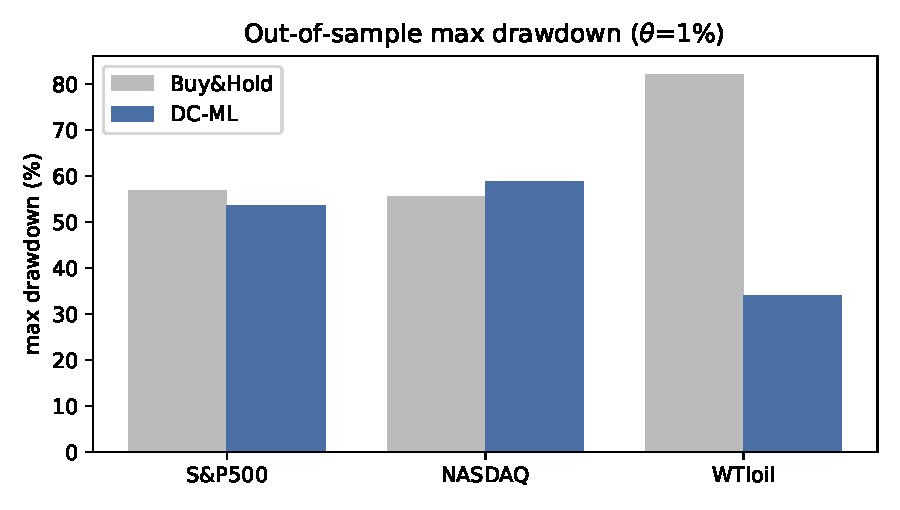
\includegraphics[width=0.7\linewidth]{fig2_drawdown.pdf}
\caption{Out-of-sample maximum drawdown, DC-ML vs Buy-and-Hold
($\theta=1\%$).}\label{fig:dd}
\end{figure}

\subsection{Cost sensitivity}
DC-ML degrades gracefully with costs but from a low base
(\texttt{results/cost\_sensitivity.csv}). On WTI it stays marginally positive
from 0 to 10\,bps/side ($+1.7\%\to+0.3\%$); on the equity indices it is negative
at every cost level ($-3.3\%\to-4.9\%$ S\&P; $-4.8\%\to-6.5\%$ NASDAQ). Crude is
the only cost-robust asset, and even there the edge is economically negligible.

\subsection{Threshold sensitivity}
Results vary strongly with $\theta$ (full grid in
\texttt{results/walkforward\_full.csv}): $\theta=1\%$ is best for WTI, but the
DC-ML annual return swings sign with $\theta$ on every asset (e.g.\ WTI is
positive only at $\theta\in\{1\%,3\%\}$ and negative elsewhere). Picking the best
$\theta$ ex post would materially overstate performance---precisely the
multiple-testing trap we set out to avoid.

\subsection{Market context and regime conditioning}
A natural objection is that the model is ``blind'' to the wider market. We
augment the DC features with market-state variables computed at each event---
20-day realised volatility, price relative to its 200-day moving average, 20-day
momentum, and drawdown-from-peak---and re-run the walk-forward. The effect is
inconsistent: context features help NASDAQ ($-5.1\%\to-2.5\%$) but hurt WTI
($+1.4\%\to-3.9\%$) and barely move S\&P ($-3.6\%\to-3.3\%$). There is no robust
``broader-picture'' gain. Conditioning the context model's out-of-sample trades
on the prevailing regime (Table~\ref{tab:regime}) is equally unconvincing: only
NASDAQ-in-bull is (marginally) positive, while every bear-market cell is
negative. No consistent regime advantage emerges.

\begin{table}[t]\centering
\caption{DC-ML ($+$context) by market regime, $\theta=1\%$, out-of-sample.}
\label{tab:regime}
\begin{tabular}{llrrr}
\toprule
Asset & Regime & Ann.\ ret & Sharpe & Hit rate \\
\midrule
S\&P500 & Bull & $-1.0\%$ & $-0.21$ & $0.40$ \\
S\&P500 & Bear & $-2.3\%$ & $-0.15$ & $0.32$ \\
NASDAQ  & Bull & $+0.8\%$ & $+0.19$ & $0.42$ \\
NASDAQ  & Bear & $-3.3\%$ & $-0.34$ & $0.32$ \\
WTI oil & Bull & $-1.3\%$ & $-0.13$ & $0.34$ \\
WTI oil & Bear & $-2.6\%$ & $-0.15$ & $0.30$ \\
\bottomrule
\end{tabular}
\end{table}

\subsection{Specification and implementation sensitivity}
Finally, the headline magnitudes are themselves fragile. An earlier draft of
this study, using a different gradient-boosting configuration, reported a DC-ML
crude-oil return of $+37.8\%$/yr (Sharpe $1.11$) and a NASDAQ result matching
buy-and-hold. Re-implementing the pipeline independently, with default
gradient-boosting hyperparameters, collapses the crude result to $+1.4\%$ and
turns NASDAQ negative---even though the \emph{qualitative} story (naive rule
loses; ML filter reduces losses and drawdown; no significant excess return) is
stable. Figure~\ref{fig:eq} shows the resulting equity curves. This sensitivity
is not a nuisance to be hidden but part of the finding: an edge that swings with
hyperparameters, implementation, asset, and regime is not an edge one should
trade.

\begin{figure}[t]\centering
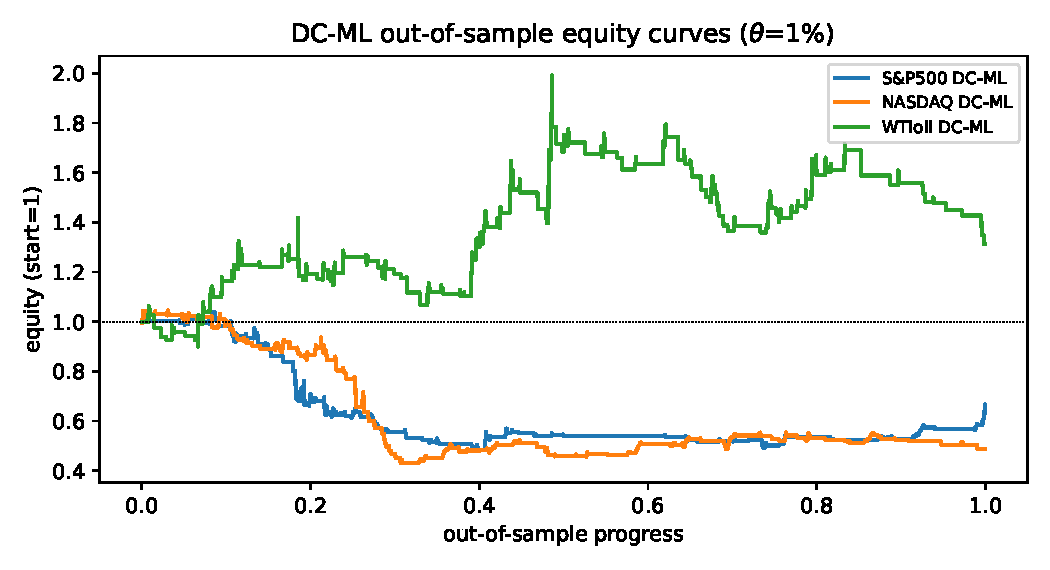
\includegraphics[width=0.8\linewidth]{fig4_equity.pdf}
\caption{DC-ML out-of-sample equity curves (walk-forward, $\theta=1\%$).}
\label{fig:eq}
\end{figure}

\section{Discussion}
The honest reading is that \emph{a DC$+$ML trading edge does not survive rigorous
out-of-sample testing} in this daily, three-asset setting. The most eye-catching
figure a DC$+$ML pipeline can produce---a fourfold crude-oil return---fails both
a significance bar ($p\approx0.21$) and, more tellingly, an independent
reimplementation, exactly the fragility that single-split backtests conceal. This
corroborates the overfitting literature within the specific context of DC
trading. Two by-products are, however, constructive. First, \emph{ML selectivity
is indispensable relative to the naive rule}: it is the difference between
catastrophic losses and roughly flat performance, achieved by declining the
great majority of low-quality signals. Second, DC-ML \emph{substantially reduces
turnover and drawdown}, indicating value as a \emph{risk-management overlay}
rather than a standalone alpha source. The feature-importance result (size of
swings matters, sign does not) further suggests that whatever signal exists is
overshoot-related, pointing future work toward overshoot dynamics rather than
directional momentum.

\section{Limitations and future work}
(i)~The strategy exits at the next DC confirmation, mechanically surrendering
$\theta$; a scaling-law- or ML-timed exit could improve net returns.
(ii)~Daily data is coarse for DC, whose strongest documented behaviour is
intraday and in FX; the pipeline ingests arbitrary CSVs, so the natural next test
is FX and crypto at higher frequency. (iii)~With ${\sim}100$--$130$
out-of-sample trades per asset, statistical power is limited. (iv)~We hold a
single position type with fixed sizing; volatility-scaled sizing and
multi-threshold ensembles are promising extensions.

\section{Conclusion}
We stress-tested a popular idea---ML filtering of directional-change trading
signals---on genuine equity and commodity data under walk-forward evaluation,
transaction costs, and bootstrap inference. The DC construction behaves as
theory predicts, and ML selectivity is clearly valuable relative to naive DC
trading, but the strategy delivers no statistically significant return and does
not match buy-and-hold on any asset; its reliable benefit is a large reduction
in turnover and drawdown. We read this as a cautionary, reproducible counterpoint
to single-split DC-trading results, and a pointer toward risk-overlay and
higher-frequency extensions.

\paragraph{Reproducibility.} Code and results:
\url{https://github.com/jarvisss007/dc-ml-trading}.
\texttt{python run\_walkforward.py} reproduces Table~\ref{tab:main};
\texttt{python extra\_analysis.py}, \texttt{context\_regime.py}, and
\texttt{plots.py} reproduce the scaling-law, feature-importance, cost,
model-comparison, regime, and figure results. Data are the three series bundled
in the \texttt{arch} package; no vendor access is required.

\begin{thebibliography}{99}
\bibitem[Arnott et al.(2019)]{arnott2019} Arnott, R., Harvey, C.R., \& Markowitz, H. (2019). A backtesting protocol in the era of machine learning. \emph{Journal of Financial Data Science}, 1(1).
\bibitem[Aloud et al.(2012)]{aloud2012} Aloud, M., Tsang, E., Olsen, R., \& Dupuis, A. (2012). A directional-change event approach for studying financial time series. \emph{Economics E-Journal}, 6.
\bibitem[Bailey et al.(2014)]{bailey2014} Bailey, D.H., Borwein, J., L\'opez de Prado, M., \& Zhu, Q.J. (2014). Pseudo-mathematics and financial charlatanism: the effects of backtest overfitting. \emph{Notices of the AMS}, 61(5).
\bibitem[Bakhach et al.(2018)]{bakhach2018} Bakhach, A., Tsang, E., \& Chinthalapati, V.L.R. (2018). TSFDC: A trading strategy based on forecasting directional change. \emph{Intelligent Systems in Accounting, Finance and Management}, 25(3).
\bibitem[Glattfelder et al.(2011)]{glattfelder2011} Glattfelder, J.B., Dupuis, A., \& Olsen, R.B. (2011). Patterns in high-frequency FX data: discovery of 12 empirical scaling laws. \emph{Quantitative Finance}, 11(4), 599--614.
\bibitem[Gu et al.(2020)]{gu2020} Gu, S., Kelly, B., \& Xiu, D. (2020). Empirical asset pricing via machine learning. \emph{Review of Financial Studies}, 33(5).
\bibitem[Guillaume et al.(1997)]{guillaume1997} Guillaume, D.M., Dacorogna, M.M., Dav\'e, R.R., M\"uller, U.A., Olsen, R.B., \& Pictet, O.V. (1997). From the bird's eye to the microscope: a survey of new stylized facts of the intra-daily foreign exchange markets. \emph{Finance and Stochastics}, 1(2).
\bibitem[Harvey \& Liu(2015)]{harvey2015} Harvey, C.R., \& Liu, Y. (2015). Backtesting. \emph{Journal of Portfolio Management}, 42(1).
\bibitem[Harvey et al.(2016)]{harvey2016} Harvey, C.R., Liu, Y., \& Zhu, H. (2016). $\ldots$ and the cross-section of expected returns. \emph{Review of Financial Studies}, 29(1).
\bibitem[Kampouridis \& Otero(2017)]{kampouridis2017} Kampouridis, M., \& Otero, F.E.B. (2017). Evolving trading strategies using directional changes. \emph{Expert Systems with Applications}, 73, 145--160.
\bibitem[L\'opez de Prado(2018)]{lopezdeprado2018} L\'opez de Prado, M. (2018). \emph{Advances in Financial Machine Learning}. Wiley.
\bibitem[Politis \& Romano(1994)]{politis1994} Politis, D.N., \& Romano, J.P. (1994). The stationary bootstrap. \emph{JASA}, 89(428), 1303--1313.
\bibitem[Tsang(2010)]{tsang2010} Tsang, E. (2010). Directional Changes, Definitions. Working Paper WP050-10, CCFEA, University of Essex.
\end{thebibliography}

\end{document}
